\section{Data Warehouse Reference Architecture}
\label{sec:referenceArchitecture}
To order to have a common understanding about the topic of Data-Warehouse-Systems it is useful to quickly elaborate their fundamentals. This will make the discussions and the considerations easier to understand.\newline
Therefore the term ''\acrshort{dws}'' will be defined and its responsibilities will be delimited. Afterwards, an architecture will be introduced which will be used as a reference during this paper.

\subsection{Defining the Data-Warehouse-System}
Before explaining the reference architecture an outlook upon the term ''data warehouse'' itself and its process is given.\newline
This term was introduced around the end of the 1980s by William H. Inmon, who is considered to be the father of this concept.
\begin{definition}
'A data warehouse is a subject-oriented, integrated, nonvolatile and time-variant collection of data in support of management's decisions.' \cite{buildingTheDWS}
\end{definition}
This results in a system which needs to be capable of retrieving, preparing and supplying data for analysis.\newline
Now let's focus on the process needed to achieve this. The official term for that is 'Data Warehousing'. It contains a process with six steps. [\cite{dwsRefArchitecture}, p. 9]
\begin{enumerate}
    \item Identify changes in relevant data form source systems
    \item Extract relevant data from those systems
    \item Integrate, transform and clean up the extracted data
    \item Load the data into the data warehouse and persist it
    \item Deploy/provide the data to analytical applications 
    \item Support to run those analysis
\end{enumerate}

\subsection{Introducing the Reference Architecture}
A system which is called data warehouse system should support and implement these steps in its software components. While developing a DWS architecture, there leads no way around discussing the most commonly used reference by A. Bauer in his book ''Data Warehouse Systems''.\cite{dwsRefArchitecture}\newline
\begin{figure}[htb]
    \centering
    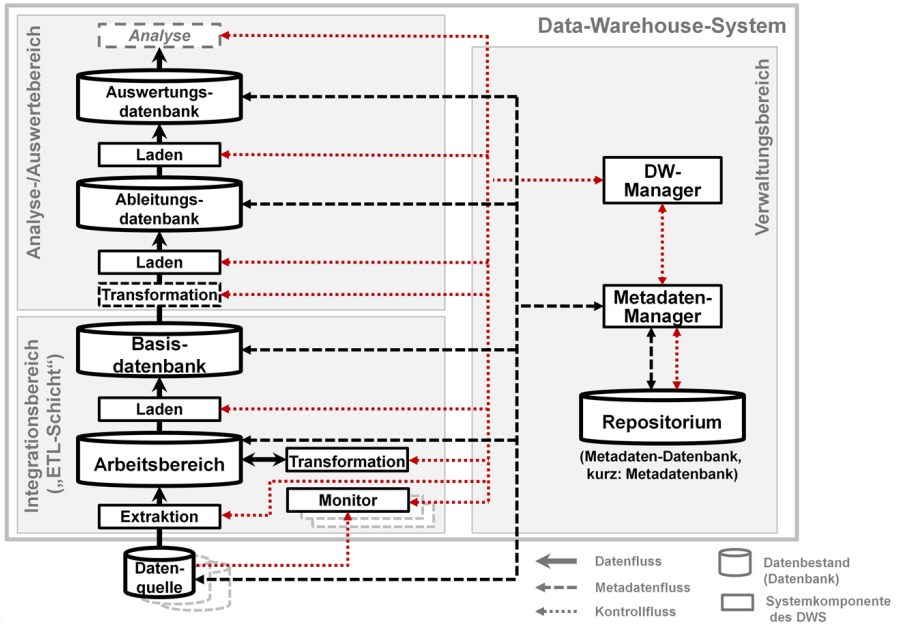
\includegraphics[scale=0.45]{pictures/DataWarehouseReferenceArchitecture.png}
    \caption{Reference architecture for data warehouse systems by A. Bauer \cite[p.~42]{dwsRefArchitecture}}
    \label{fig:referenceArchitecture}
\end{figure} 

Now the pictured software components and databases from figure \ref{fig:referenceArchitecture} quickly  will be gone through starting at the bottom of the \acrfull{etl} layer. In order to retrieve data from several source systems with distinct technologies, a complex extraction component is needed. This can be triggered by a monitor which scans for data changes in those data sources.\newline
After this step, the whole data is loaded into a staging area in which a transformation is performed. Two buzzwords in this context are data cleaning and cleansing. Therefore, the more complex data cleansing will be elaborated.
''Data cleansing is the act of correcting or moving inaccurate, broken, or erroneous data from your data-set.'' \cite{dataCleansing}
This step results in the Core data warehouse, which is basically a database containing all historic, cleaned, consolidated and analysis-neutral data samples. In conclusion, we can speak of an ''single source of truth''\cite{scriptRasch}, which is a centralised and integrated database used as the basis for further data handling and analysis.\newline
\\
The next part focuses on the analytical layer of the reference architecture. All data will be loaded from the core database into the derivation database. This database is redundant to the core database but contains additional non-analysis-neutral derived data. Upon this database the data marts are build. Data marts are a slice of the entire data. Additionally, it is focused on analysis and therefore has other data structures. In most use cases, multiple of these exist in order to have fast and detailed analysis of different areas inside a possible institution.\newline
\\
On the right side of figure \ref{sec:referenceArchitecture} the management layer is visualised. It contains components for managing the sequence- and data flow and the metadata repository itself. 
% The metadata repository contains all the information regarding the state of the data warehouse. The managing component works with those in order to control the system.
\newline
\\
This should have described the fundamental ideas and concepts of a data warehouse system without going into depths. The shown approach is closely related to Inmon's hub and spoke architecture which will be introduced in the next section. 
